\documentclass[../notes.tex]{subfiles}

\pagestyle{main}
\renewcommand{\chaptermark}[1]{\markboth{\chaptername\ \thechapter\ (#1)}{}}
\stepcounter{chapter}

\begin{document}




\chapter{The Schr\"{o}dinger Equation}
\section{Ehrenfest Theorem and Uncertainty Principle}
\begin{itemize}
    \item \marginnote{1/8:}Announcement: PSet 1 due Friday at midnight.
    \item Recap.
    \begin{itemize}
        \item $\psi(\vec{r},t)$ is a wave function to which we associate a \textbf{probability density}.
        \begin{itemize}
            \item Integrating this probability density over a volume yields the probability that the particle is in $V$.
            \item Moreover, $\psi$ is not arbitrary but must satisfy the Schr\"{o}dinger equation.
        \end{itemize}
        \item $\hat{\vec{p}}$ is the momentum operator, defined as the differential operator $-i\hbar\vec{\nabla}$.
        \item Expressing the Schr\"{o}dinger equation in terms of $\hat{\vec{p}}$, we see that it represents the application of a Hamiltonian operator in the usual form from last quarter (i.e., kinetic plus potential energy) to a certain function.
        \item $\Exp{\hat{\vec{r}}\,}$ is the mean position, and $\Exp{\hat{\vec{p}}\,}$ is the mean momentum.
        \begin{itemize}
            \item The mean position and mean momentum satisfy the classical relation, i.e., $\dd{\Exp{\hat{\vec{r}}\,}}/\dd{t}=\Exp{\hat{\vec{p}}\,}/m$.
        \end{itemize}
    \end{itemize}
    \item \textbf{Probability density}: The quantity given as follows. \emph{Given by}
    \begin{equation*}
        |\psi(\vec{r},t)|^2
    \end{equation*}
    \item We now prove something even more amazing than the classical relation result: An analogy to the classical Newton's law.
    \item \textbf{Ehrenfest's theorem}: The time derivative of the expectation value of the momentum operator is related to the expectation value of the force $F:=-\vec{\nabla}V$ on a massive particle moving in a scalar potential $V(\vec{r},t)$ as follows.
    \begin{equation*}
        \dv{\Exp{\hat{\vec{p}}\,}}{t} = \Exp{-\vec{\nabla}V(\vec{r},t)}
    \end{equation*}
    \begin{proof}
        Consider the Schr\"{o}dinger equation:
        \begin{equation*}
            -i\hbar\pdv{\psi}{t} = \frac{\hbar^2}{2m}\vec{\nabla}^2\psi-V(\vec{r},t)\psi
        \end{equation*}
        Take the complex conjugate of it. This means that we're sending $i\mapsto -i$, keeping $V$ fixed (it's real), and sending $\psi\mapsto\psi^*$ (the inclusion of $i$ in the Schr\"{o}dinger equation means that $\psi$ is complex in general and thus has a nontrivial complex conjugate).
        \begin{equation*}
            -i\hbar\pdv{\psi^*}{t} = -\frac{\hbar^2}{2m}\vec{\nabla}^2\psi^*+V(\vec{r},t)\psi^*
        \end{equation*}
        Also observe that
        \begin{equation*}
            \int\dd^3\vec{r}\ \psi^*\vec{\nabla}(\vec{\nabla}^2\psi) = \int\dd^3\vec{r}\ \vec{\nabla}\cdot[\psi^*\vec{\nabla}^2\psi]-\int\dd^3\vec{r}\ \vec{\nabla}\psi^*\vec{\nabla}^2\psi
            = -\int\dd^3\vec{r}\ \vec{\nabla}\psi^*\vec{\nabla}^2\psi
        \end{equation*}
        where the first term goes to zero by the divergence theorem and the boundary condition. (See PSet 1, Q2a for a full explanation of this zeroing out.) Similarly, we have that
        \begin{equation*}
            \int\dd^3\vec{r}\ \vec{\nabla}\psi^*\vec{\nabla}(\vec{\nabla}\psi) = -\int\dd^3\vec{r}\ \vec{\nabla}^2\psi^*\vec{\nabla}\psi
        \end{equation*}
        This means that altogether,
        \begin{align*}
            \int\dd^3\vec{r}\ \psi^*\vec{\nabla}^3\psi &= \int\dd^3\vec{r}\ \vec{\nabla}^2\psi^*\vec{\nabla}\psi\\
            \int\dd^3\vec{r}\ [\vec{\nabla}^2\psi^*\vec{\nabla}\psi-\psi^*\vec{\nabla}^3\psi] &= 0
        \end{align*}
        We will now use the two Schr\"{o}dinger substitutions and the above equation to substitute into the following algebraic derivation.
        \begin{align*}
            \dv{\Exp{\hat{\vec{p}}\,}}{t} ={}& \dv{t}(\int\dd^3\vec{r}\ \psi^*(-i\hbar\vec{\nabla}\psi))\\
            ={}& \int\dd^3\vec{r}\ {\pdv{\psi^*}{t}}(-i\hbar\vec{\nabla}\psi)+\int\dd^3\vec{r}\ \psi^*\left( -i\hbar\vec{\nabla}\pdv{\psi}{t} \right)\\
            ={}& \int\dd^3\vec{r}\,\left( -i\hbar{\pdv{\psi^*}{t}} \right)(\vec{\nabla}\psi)+\int\dd^3\vec{r}\ \psi^*\vec{\nabla}\left( -i\hbar\pdv{\psi}{t} \right)\\
            \begin{split}
                ={}& \int\dd^3\vec{r}\,\left( -\frac{\hbar^2}{2m}\vec{\nabla}^2\psi^*+V(\vec{r},t)\psi^* \right)(\vec{\nabla}\psi)\\
                & +\int\dd^3\vec{r}\ \psi^*\vec{\nabla}\left( \frac{\hbar^2}{2m}\vec{\nabla}^2\psi-V(\vec{r},t)\psi \right)
            \end{split}\\
            \begin{split}
                ={}& \int\dd^3\vec{r}\,\left[ -\frac{\hbar^2}{2m}\vec{\nabla}^2\psi^*(\vec{\nabla}\psi) \right]+\int\dd^3\vec{r}\ \psi^*\vec{\nabla}\left( \frac{\hbar^2}{2m}\vec{\nabla}^2\psi \right)\\
                & +\int\dd^3\vec{r}\,\left[ V(\vec{r},t)\psi^*(\vec{\nabla}\psi)+\psi^*\vec{\nabla}[-V(\vec{r},t)\psi] \right]
            \end{split}\\
            \begin{split}
                ={}& \int\dd^3\vec{r}\ -\frac{\hbar^2}{2m}\left[ \vec{\nabla}^2\psi^*(\vec{\nabla}\psi)-\psi^*\vec{\nabla}^3\psi \right]\\
                & +\int\dd^3\vec{r}\,\left[ V(\vec{r},t)\psi^*(\vec{\nabla}\psi)-\psi^*\vec{\nabla}[V(\vec{r},t)]\psi-\psi^*V(\vec{r},t)(\vec{\nabla}\psi) \right]
            \end{split}\\
            ={}& \int\dd^3\vec{r}\ \psi^*(-\vec{\nabla}V(\vec{r},t))\psi\\
            ={}& \Exp{-\vec{\nabla}V(\vec{r},t)}
        \end{align*}
        as desired.
    \end{proof}
    \item In quantum mechanics, we have \textbf{observables} which are in one-to-one correspondence with operators.
    \begin{table}[H]
        \centering
        \small
        \renewcommand{\arraystretch}{1.4}
        \begin{tabular}{c|c}
            \textbf{Observables} & \textbf{Operators ($\bm{\hat{O}}$)}\\
            \hline
            $\vec{r}$ & $\hat{\vec{r}}$\\
            $V(\vec{r},t)$ & $\hat{V}(\vec{r},t)$\\
            $\hat{\vec{p}}$ & $-i\hbar\vec{\nabla}$\\
            $\hat{H}$ & $-\dfrac{\hbar^2}{2m}\vec{\nabla}^2+V(\vec{r},t)$\\
        \end{tabular}
        \caption{Observables vs. operators.}
        \label{tab:observablesOperators}
    \end{table}
    \begin{itemize}
        \item Recall that any Hermitian operator has a real observable.
    \end{itemize}
    \item Define
    \begin{equation*}
        \hat{O}_{ij} := \int\dd^3\vec{r}\ \psi_i^*\hat{O}\psi_j
    \end{equation*}
    \begin{itemize}
        \item Then note that
        \begin{equation*}
            \hat{O}_{ij} = (\hat{O}_{ji})^*
        \end{equation*}
        \item Thus, an equivalent definition of a Hermitian operator is one such that the above equation is satisfied for all relevant $i,j$.
    \end{itemize}
    \item Recall that the Schr\"{o}dinger equation is linear.
    \begin{itemize}
        \item Let $\psi=\sum_ic_i\psi_i$.
        \item Then
        \begin{equation*}
            \int\dd^3\vec{r}\ \psi^*\hat{O}\psi = \sum_{i,j}\int\dd^3\vec{r}\ c_i^*\psi_i^*\hat{O}c_j\psi_j
            = \sum_{i,j}c_i^*c_j\hat{O}_{ij}
        \end{equation*}
        is real.
        \item Takeaway: Averages over arbitrary wavefunctions are real.
        \item Similarly, suppose that $\vec{r}$ is Hermitian. Then any function $V(\vec{r})$ of it is also Hermitian.
        \item For example, the momentum operator is a Hermitian operator:
        \begin{equation*}
            \int\dd^3\vec{r}\ \psi_i^*(-i\hbar\vec{\nabla}\psi_j) = \left( \int\dd^3\vec{r}\ \psi_j^*(-i\hbar\vec{\nabla}\psi_i) \right)^*
            = \int\dd^3\vec{r}\ \psi_j(i\hbar\vec{\nabla}\psi_i^*)
            \to -\int\dd^3\vec{r}\ \vec{\nabla}\psi_j(i\hbar\psi_i^*)
        \end{equation*}
        \item To prove the leftmost equality above, we can use integration by parts as follows.
        \begin{align*}
            \int\dd^3\vec{r}\ \psi_j(i\hbar\vec{\nabla}\psi_i^*) &= i\hbar\int\dd^3\vec{r}\ \vec{\nabla}(\psi_j\psi_i^*)-\int\dd^3\vec{r}\ \vec{\nabla}\psi_j(i\hbar\psi_i^*)\\
            &= i\hbar\vec{\nabla}\int\dd^3\vec{r}\ (\psi_j\psi_i^*)-\int\dd^3\vec{r}\ \vec{\nabla}\psi_j(i\hbar\psi_i^*)\\
            &= i\hbar\vec{\nabla}0-\int\dd^3\vec{r}\ \vec{\nabla}\psi_j(i\hbar\psi_i^*)\\
            &= -\int\dd^3\vec{r}\ \vec{\nabla}\psi_j(i\hbar\psi_i^*)
        \end{align*}
        \begin{itemize}
            \item Note that the left integral above goes to zero because of the boundary condition.
            \item This is relevant to PSet 1, Q2a!
        \end{itemize}
    \end{itemize}
    \item Linear algebra analogy.
    \begin{itemize}
        \item Recall that we can write any vector $\vec{v}$ componentwise as $\vec{v}=v_x\vec{x}+v_y\vec{y}+v_z\vec{z}$.
        \item We can apply matrices $A$ to such vectors to generate other vectors via $A\vec{v}=\vec{v}{\,}'$ and the like.
        \item Lastly, we have an inner product $\cdot$ such that $\vec{a}\cdot\vec{b}=\delta_{ab}$, where $a,b=x,y,z$.
        \item On an infinite-dimensional vector space, such as that containing all the $\psi$, we still can decompose $\psi=\sum_nc_n\psi_n$ into an infinite sum of basis components, apply operators $\hat{O}\psi=\psi'$, and have an inner product $\int\dd^3\vec{r}\ \psi^*_m\psi_n=\delta_{mn}$.
        \item Another analogy: Like the inner product of a vector and unit vector is the component of the vector in that direction (e.g., $\vec{v}\cdot\vec{x}=v_x$), we have
        \begin{equation*}
            \int\dd^3\vec{r}\ \psi_m^*\psi = \int\dd^3\vec{r}\psi_m^*\sum_nc_n\psi_n = c_m
        \end{equation*}
        \item One more analogy: $\vec{x}^TA\vec{x}=A_{xx}$ is like $\ev{\hat{O}}{\psi_i}=\hat{O}_{ii}$.
    \end{itemize}
\end{itemize}



\section{Time-Independent Potentials}
\begin{itemize}
    \item \marginnote{1/10:}Recap of important equations.
    \begin{itemize}
        \item Momentum and Hamiltonian operators.
        \item Schr\"{o}dinger equation.
        \item Expectation values of $\vec{x}$ and $\vec{p}$, the classical relation between them, and Ehrenfest's theorem.
        \item Hermitian operator condition.
        \begin{itemize}
            \item The fact that their observables are real.
            \item Examples: $\hat{\vec{p}}$, $\hat{H}$, $\hat{\vec{p}}{\,}^2/2m$, $V(\vec{r},t)$.
        \end{itemize}
    \end{itemize}
    \item \textbf{Adjoint} (of $\hat{O}$): The operator defined according to the following rule. \emph{Denoted by} $\bm{\hat{O}^\dagger}$. \emph{Constraint}
    \begin{equation*}
        \int\dd^3\vec{r}\ \psi_i^*\hat{O}\psi_j = \int\dd^3\vec{r}\ (\hat{O}^\dagger\psi_i)^*\psi_j
    \end{equation*}
    \begin{itemize}
        \item A self-adjoint (Hermitian) operator is an operator satisfying $\hat{O}=\hat{O}^\dagger$.
    \end{itemize}
    \item Dirac notation.
    \begin{itemize}
        \item Associate with each $\psi(\vec{r},t)$ a "ket" $\ket{\psi}$ and a "bra" $\bra{\psi}$.
        \begin{itemize}
            \item These are like vectors.
        \end{itemize}
        \item The full "bra-ket" $\braket{\psi_i}{\psi_j}:=\int\dd^3\vec{r}\ \psi_i^*\psi_j$.
        \item We also have $\mel{\psi_i}{\hat{O}}{\psi_j}:=\int\dd^3\vec{r}\ \psi_i^*\hat{O}\psi_j$.
        \item Essentially, we're just representing this Hilbert-space integral inner product in typical inner product notation!
    \end{itemize}
    \item The condition for an operator being Hermitian/self-adjoint in Dirac notation:
    \begin{equation*}
        \mel{\psi_i}{\hat{O}}{\psi_j} = \braket{\psi_i}{\hat{O}\psi_j}
        = \braket{\hat{O}^\dagger\psi_i}{\psi_j}
    \end{equation*}
    \item We also have that
    \begin{equation*}
        \mel{\psi_i}{\hat{O}_1\hat{O}_2}{\psi_j} = \braket{\psi_i}{\hat{O}_1\hat{O}_2\psi_j}
        = \braket{\hat{O}_1^\dagger\psi_i}{\hat{O}_2\psi_j}
        = \braket{\hat{O}_2^\dagger\hat{O}_1^\dagger\psi_i}{\psi_j}
    \end{equation*}
    \begin{itemize}
        \item This is very relevant to PSet 1, Q3a!
    \end{itemize}
    \item Dirac notation allows us to represent complicated expressions such as
    \begin{equation*}
        \int\dd^3\vec{r}\ {\psi'}^*\psi = \left( \int\dd^3\vec{r}\ \psi^*\psi' \right)^*
    \end{equation*}
    in the form
    \begin{equation*}
        \braket{\psi}{\psi'} = \left( \braket{\psi'}{\psi} \right)^*
    \end{equation*}
    \item In Dirac notation, the Hermitian condition becomes
    \begin{equation*}
        \braket{\psi_i}{\hat{O}_1\hat{O}_2\psi_j} = \braket{\hat{O}_2\hat{O}_1\psi_i}{\psi_j}
    \end{equation*}
    \item We also have that
    \begin{equation*}
        \braket{\psi_i}{\hat{O}_1\hat{O}_2\psi_j} = \left( \braket{\psi_j}{\hat{O}_2\hat{O}_1\psi_i} \right)^*
    \end{equation*}
    \begin{itemize}
        \item This is also relevant to PSet 1, Q3a!
    \end{itemize}
    \item This last statement has some consequences.
    \begin{itemize}
        \item In particular, if $\psi_i=\psi_j=\psi$, then
        \begin{equation*}
            \braket{\psi}{\hat{O}_1\hat{O}_2\psi} = \left( \braket{\psi}{\hat{O}_2\hat{O}_1\psi} \right)^*
        \end{equation*}
        \item Thus, by adding and subtracting the quantities in the above result, we learn that
        \begin{equation*}
            \braket{\psi}{(\hat{O}_1\hat{O}_2-\hat{O}_2\hat{O}_1)\psi}
        \end{equation*}
        is an imaginary number and
        \begin{equation*}
            \braket{\psi}{(\hat{O}_1\hat{O}_2+\hat{O}_2\hat{O}_1)\psi}
        \end{equation*}
        is a real number.
    \end{itemize}
    \item Example: The commutator of the position and momentum operators gives a purely imaginary number.
    \begin{itemize}
        \item We have that
        \begin{equation*}
            [\hat{\vec{p}}_x,\hat{x}]f = (\hat{\vec{p}}_xx-x\hat{\vec{p}}_x)f
            = -i\hbar\pdv{x}(xf)+xi\hbar\pdv{f}{x}
            = -i\hbar\pdv{x}{x}f-i\hbar x\pdv{f}{x}+i\hbar x\pdv{f}{x}
            = -i\hbar f
        \end{equation*}
        \item Thus,
        \begin{equation*}
            [\hat{\vec{p}}_x,\hat{x}] = -i\hbar
        \end{equation*}
        as desired.
    \end{itemize}
    \item Can $\psi_n$ be an eigenstate of $\hat{O}_1$ and $\hat{O}_2$ simultaneously?
    \begin{itemize}
        \item In the mold of a typical eigenvalue equation $A\vec{x}_n=\lambda_n\vec{x}_n$, let
        \begin{align*}
            \hat{O}\psi_n &= O_n\psi_n&
            \hat{O}_1\psi_n &= O_{1,n}\psi_n&
            \hat{O}_2\psi_m' &= O_{2,m}\psi_m'
        \end{align*}
        \item Then we have that
        \begin{align*}
            \hat{O}_1\psi_n &= O_{1,n}\psi_n\\
            \hat{O}_2\hat{O}_1\psi_n &= O_{1,n}\hat{O}_2\psi_n = O_{1,n}O_{2,n}\psi_n
        \end{align*}
        and
        \begin{align*}
            \hat{O}_2\psi_n &= O_{2,n}\psi_n\\
            \hat{O}_1\hat{O}_2\psi_n &= O_{2,n}\hat{O}_1\psi_n = O_{2,n}O_{1,n}\psi_n
        \end{align*}
        \item These are the relevant constraints.
        \item If such a $\psi_n$ exists, then we can determine the values of $\hat{O}_1,\hat{O}_2$ simultaneously to infinite precision.
    \end{itemize}
    \item The commutator is associated with a compatible observable.
    \begin{itemize}
        \item In particular, when two operators commute, we say that the associated physical observables are \textbf{compatible}.
    \end{itemize}
    \item Because waves move in a \textbf{wave packet}, there is some uncertainty in the position.
    \begin{itemize}
        \item In particular, the uncertainty of $\hat{A}$ in a given state $\psi$ is
        \begin{equation*}
            \ev{(\hat{A}-\Exp{\hat{A}})^2}{\psi}
        \end{equation*}
        \item An alternate form of this expression is
        \begin{equation*}
            \ev{\Exp{\hat{A}^2}-\Exp{\hat{A}}^2}{\psi}
        \end{equation*}
        \begin{itemize}
            \item Wagner proves this as in MathChapter B from CHEM26100Notes.
        \end{itemize}
    \end{itemize}
    \item \textbf{Wave packet}: It is a continuous sum of waves of different frequencies.
    \item If $\psi_n$ is an eigenstate of $\hat{A}$\dots
    \begin{itemize}
        \item Then
        \begin{equation*}
            \ev{\hat{A}}{\psi_n} = A_n\braket{\psi_n} = A_n
        \end{equation*}
        \item Similarly,
        \begin{equation*}
            \ev{\hat{A}^2}{\psi_n} = A_n^2\braket{\psi_n} = A_n^2
        \end{equation*}
        \item Therefore, the uncertainty of $\hat{A}$ in an eigenstate is $A_n^2-(A_n)^2=0$.
    \end{itemize}
    \item Note that the condition "$\psi$ is an eigenstate of $\hat{A}$" can be denoted via $\hat{A}\ket{\psi_n}=A_n\ket{\psi_n}$.
    \item \textbf{Heisenberg uncertainty principle}. \emph{Given by}
    \begin{equation*}
        \sigma_x\sigma_{p_x} \geq \frac{\hbar}{2}
    \end{equation*}
    \item Why is this the case? It is related to $[p_x,x]=-i\hbar$.
    \begin{itemize}
        \item The full derivation is in the notes (transcribed below), but for now, know that it is a general fact that
        \begin{equation*}
            \sigma_A^2\sigma_B^2 \geq \frac{1}{4}|\ev{[A,B]}{\psi}|^2
        \end{equation*}
        \item We demonstrate this via the \textbf{Schwarz inequality}.
        \item One thing is always complex; the other is always real.
    \end{itemize}
    \item \textbf{Cauchy-Schwarz inequality}. \emph{Given by}
    \begin{equation*}
        (f,f)(g,g) \geq |(f,g)|^2
    \end{equation*}
    \begin{itemize}
        \item $(f,g)$ denotes the inner product of $f$ and $g$, where $f,g$ are elements of an abstract vector space.
    \end{itemize}
    \item \textbf{Schwarz inequality}. \emph{Given by}
    \begin{equation*}
        \left( \int\dd^3\vec{r}\ |f|^2 \right)\left( \int\dd^3\vec{r}\ |g|^2 \right) \geq \left| \int\dd^3\vec{r}\ fg^* \right|^2
    \end{equation*}
    \begin{itemize}
        \item In Dirac's notation, this is
        \begin{equation*}
            \braket{f}\cdot\braket{g} \geq |\braket{f}{g}|^2
        \end{equation*}
    \end{itemize}
    \item Full derivation of the Heisenberg uncertainty principle.
    \begin{itemize}
        \item Apply the Schwarz inequality to $f=(\hat{A}-\Exp{\hat{A}})\psi$ and $g=(\hat{B}-\Exp{\hat{B}})\psi$, for $\hat{A},\hat{B}$ Hermitian.
        \item Recall that the following identities hold for Hermitian/self-adjoint operators.
        \begin{align*}
            \mel{\psi}{\hat{A}}{\psi'} &= \braket{\psi}{\hat{A}\psi'} = \braket{\hat{A}\psi}{\psi'}&
            \mel{\psi}{\hat{A}^2}{\psi'} &= \braket{\hat{A}\psi}{\hat{A}\psi'}
        \end{align*}
        \item Consequently, we have that
        \begin{align*}
            \sigma_A^2\cdot\sigma_B^2 &= \ev{(\hat{A}-\Exp{\hat{A}})^2}{\psi}\cdot\ev{(\hat{B}-\Exp{\hat{B}})^2}{\psi}\\
            &= \braket{(\hat{A}-\Exp{\hat{A}})\psi}{(\hat{A}-\Exp{\hat{A}})\psi}\cdot\braket{(\hat{B}-\Exp{\hat{B}})\psi}{(\hat{B}-\Exp{\hat{B}})\psi}\\
            &\geq \left| \braket{(\hat{A}-\Exp{\hat{A}})\psi}{(\hat{B}-\Exp{\hat{B}})\psi} \right|^2\\
            &= \Big| \ev{(\underbrace{\hat{A}-\Exp{\hat{A}}}_{\Delta\hat{A}})(\underbrace{\hat{B}-\Exp{\hat{B}}}_{\Delta\hat{B}})}{\psi} \Big|^2
            \intertext{Now, any product of operators can be expressed as one half of the sum of the \textbf{commutator} and the \textbf{anticommutator}. Thus, continuing,}
            &= \Big| \ev{\frac{1}{2}([\Delta\hat{A},\Delta\hat{B}]+\{\Delta\hat{A},\Delta\hat{B}\})}{\psi} \Big|^2\\
            &= \frac{1}{4}\Big| \ev{[\Delta\hat{A},\Delta\hat{B}]+\{\Delta\hat{A},\Delta\hat{B}\}}{\psi} \Big|^2
            \intertext{Recall from above that the mean value of the commutator is an imaginary number and the mean value of the anticommutator is a real number. Thus, if we split the above equation into two terms, the mean value of the anticommutator will be squared, hence a positive number that we can get rid of and maintain the inequality. Lastly, we can compute that $[\Delta\hat{A},\Delta\hat{B}]=[\hat{A},\hat{B}]$. Therefore,}
            &\geq \frac{1}{4}\Big| \ev{[\hat{A},\hat{B}]}{\psi} \Big|^2
        \end{align*}
        \item Example: Since $[p_x,x]=-i\hbar$, we can recover the Heisenberg uncertainty principle from the above inequality.
        \item There's some stuff in the notes that is very relevant to PSet 1, Q3b.
    \end{itemize}
    \item \textbf{Commutator} (of $\hat{O}_1,\hat{O}_2$): The operator defined as follows. \emph{Denoted by} $\bm{[\hat{O}_1,\hat{O}_2]}$. \emph{Given by}
    \begin{equation*}
        [\hat{O}_1,\hat{O}_2] = \hat{O}_1\hat{O}_2-\hat{O}_1\hat{O}_2
    \end{equation*}
    \item \textbf{Anticommutator} (of $\hat{O}_1,\hat{O}_2$): The operator defined as follows. \emph{Denoted by} $\bm{\{\hat{O}_1,\hat{O}_2\}}$. \emph{Given by}
    \begin{equation*}
        \{\hat{O}_1,\hat{O}_2\} = \hat{O}_1\hat{O}_2+\hat{O}_2\hat{O}_1
    \end{equation*}
\end{itemize}



\section{Office Hours (Matt)}
\begin{itemize}
    \item PSet 1, Q2a: Conceptual reason why the first term in the integration by parts vanishes?
    \begin{itemize}
        \item Boundary conditions in each of the three directional integrals.
    \end{itemize}
    \item Quite heavily attended, but Matt still got around.
\end{itemize}



\section{Discussion Section}
\begin{itemize}
    \item There's not that much content to go over today, so we'll talk about some more mathematical tools like the Dirac delta function and Fourier transforms.
    \item \textbf{Dirac delta function}: The function defined as follows. \emph{Denoted by} $\bm{\delta(x-x_0)}$. \emph{Given by}
    \begin{equation*}
        \delta(x-x_0) =
        \begin{cases}
            \infty & x=x_0\\
            0 & x\neq x_0
        \end{cases}
    \end{equation*}
    \item Useful for solving the Schr\"{o}dinger equation; this is a potential that we'll solve for.
    \item Important application:
    \begin{equation*}
        \int_a^b\dd{x}\delta(x-x_0)f(x) =
        \begin{cases}
            f(x_0) & x_0\in[a,b]\\
            0 & \text{otherwise}
        \end{cases}
    \end{equation*}
    \item Examples.
    \begin{enumerate}
        \item 
        \begin{equation*}
            \int_{-5}^5\dd{x}\delta(x+4)(x^2-3x+4) = \eval{x^2-3x+4}_{x=-4}
            = 32
        \end{equation*}
        \item 
        \begin{equation*}
            \int_0^\infty\delta(x+\pi)\cos(x) = 0
        \end{equation*}
        \begin{itemize}
            \item Because $x_0=-\pi\notin[0,\infty)$.
        \end{itemize}
    \end{enumerate}
    \item Defining a notion of equality.
    \begin{itemize}
        \item Let $D_1(x),D_2(x)$ be functions of the $\delta$-function.
        \begin{itemize}
            \item Example: $D_1(x)=\delta(x+3)\e[-3x^2]$.
        \end{itemize}
        \item We say that $D_1(x)=D_2(x)$ if
        \begin{equation*}
            \int_{-\infty}^\infty\dd{x}D_1(x)f(x) = \int_{-\infty}^\infty\dd{x}D_2(x)f(x)
        \end{equation*}
        for any smooth function $f$.
    \end{itemize}
    \item $\delta$-function equalities.
    \begin{enumerate}
        \item $x\delta(x)=0$.
        \item $\delta(x)=\delta(-x)$.
        \item $\delta(cx)=\frac{1}{|c|}\delta(x)$.
        \item $\int_{-\infty}^\infty\dd{x}\delta(a-x)\delta(x-b)=\delta(a-b)$.
        \item $g(x)\delta(x-a)=g(a)\delta(x-a)$.
    \end{enumerate}
    \item These equalities will probably come in handy when we start working with the $\delta$-function.
    \item We can prove these five equalities with the notion of equality defined above.
    \item Example: Proving equality 1.
    \begin{proof}
        Let $D_1(x)=x\delta(x)$ and $D_2(x)=0$. Then
        \begin{equation*}
            \int_{-\infty}^\infty\dd{x}\delta(x)xf(x) = \eval{xf(x)}_{x=0} = 0
        \end{equation*}
        and
        \begin{equation*}
            \int_{-\infty}^\infty\dd{x}0f(x) = 0
        \end{equation*}
        It follows by transitivity that the two integrals equal each other, so we must have $x\delta(x)=0$ as desired.
    \end{proof}
    \item Equality 4 is the hardest to prove. We will have a constant $D_1(x)$ equal to
    \begin{equation*}
        D_1(x) = \int_{-\infty}^\infty\dd{y}\delta(a-y)\delta(y-b)
    \end{equation*}
    \item Fourier transforms (FT) of $\delta$-functions.
    \item Recall:
    \begin{itemize}
        \item The FT of the function $\phi(x)$ is
        \begin{equation*}
            \tilde{\phi}(k) := \frac{1}{\sqrt{2\pi}}\int_{-\infty}^\infty\dd{x}\e[-ikx]\phi(x)
        \end{equation*}
        \item The inverse FT is
        \begin{equation*}
            \phi(x) := \frac{1}{\sqrt{2\pi}}\int_{-\infty}^\infty\dd{k}\e[ikx]\tilde{\phi}(k)
        \end{equation*}
    \end{itemize}
    \item We call the FT of $\delta(x-x_0)$ the function
    \begin{equation*}
        \tilde{\phi}(k;x_0) = \frac{1}{\sqrt{2\pi}}\int_{-\infty}^\infty\dd{x}\e[-ikx]\delta(x-x_0)
        = \eval{\frac{1}{\sqrt{2\pi}}\e[-ikx]}_{x=x_0}
        = \frac{1}{\sqrt{2\pi}}\e[-ikx_0]
    \end{equation*}
    \item In addition:
    \begin{align*}
        \delta(x) &= \frac{1}{2\pi}\int_{-\infty}^\infty\dd{k}\e[ikx]&
        \tilde{\delta}(k) &= \frac{1}{2\pi}\int_{-\infty}^\infty\dd{x}\e[-ikx]
    \end{align*}
    \item Matt explains the FT in terms of decomposing sums of sines and cosines.
    \item Now the physics starts!
    \item Expectation values.
    \item So far, we have the wavefunction $\psi(x)$, which mysteriously contains information on the particle.
    \begin{itemize}
        \item It solves the Schr\"{o}dinger equation.
    \end{itemize}
    \item $|\psi(x)|^2$ gives the probability density of finding the particle at $x$.
    \item The expectation value of some function $f(x)$ is
    \begin{equation*}
        \Exp{f(x)} = \int_{-\infty}^\infty\dd{x}\psi^*(x)f(x)\psi(x)
    \end{equation*}
    \item 1D momentum $\hat{p}$ can be written as the operator $-i\hbar\pdv*{x}$. Thus,
    \begin{equation*}
        \Exp{p} = \int_{-\infty}^\infty\dd{x}\psi^*
        = \int_{-\infty}^\infty\dd{x}\psi^*\left( -i\hbar\pdv{\psi}{x} \right)
    \end{equation*}
    \begin{itemize}
        \item This holds for $n^\text{th}$ powers:
        \begin{equation*}
            \Exp{\hat{p}^n} = \int_{-\infty}^\infty\dd{x}\psi^*(-i\hbar)^n\pdv[n]{\psi}{x}
        \end{equation*}
    \end{itemize}
    \item Example (PSet 1, Q2): Prove that
    \begin{equation*}
        \Exp{f(p)} = \int_{-\infty}^\infty\dd{k}f(\hbar k)|\tilde{\psi}(k)|^2
    \end{equation*}
    \begin{proof}
        Start from
        \begin{equation*}
            \Exp{f(p)} = \int_{-\infty}^\infty\dd{x}\psi^*(x)f(p)\psi(x)
        \end{equation*}
        Taylor expand about $f(0)$:
        \begin{align*}
            f(p) &= f(0)+\eval{\pdv{f}{p}}_{p=0}p+\frac{1}{2!}\eval{\pdv[2]{f}{p}}_{p=0}p^2+\cdots
            = \sum_{n=0}^\infty\frac{1}{n!}\eval{\pdv[n]{f}{p_n}}_{p=0}\\
            &= \int_{-\infty}^\infty\dd{x}\psi^*(x)\sum_{n=0}^\infty\frac{1}{n!}\eval{\pdv[n]{f}{p}}_{p=0}p^n\psi(x)\\
            &= \sum_{n=0}^\infty\frac{1}{n!}\eval{\pdv[n]{f}{p}}_{p=0}\int_{-\infty}^\infty\dd{x}\psi^*(x)p^n\psi(x)\\
            &= \sum_{n=0}^\infty\frac{1}{n!}\eval{\pdv[n]{f}{p}}_{p=0}\Exp{p^n}
        \end{align*}
        This holds when
        \begin{align*}
            \Exp{p^n} &= \int_{-\infty}^\infty\dd{x}\psi^*(x)(-i\hbar)^n\pdv[n]{\psi}{x}\\
            &= \int_{-\infty}^\infty\dd{x}\left( \frac{1}{\sqrt{2\pi}}\int_{-\infty}^\infty\dd{k}\e[ikx]\psi(x) \right)^*(-i\hbar)^n\pdv[n]{x}(\frac{1}{\sqrt{2\pi}}\int_{-\infty}^\infty\dd{\ell}\e[i\ell x]\tilde{\psi}(\ell))\\
            &= \frac{(-i\hbar)^n}{2\pi}\int_{-\infty}^\infty\dd{x}\int_{-\infty}^\infty\dd{k}\int_{-\infty}^\infty\dd{\ell}\e[-ikx]\tilde{\psi}^*(k)\tilde{\psi}(\ell)\pdv[n]{x}(\e[i\ell x])\\
            &= \frac{(-i\hbar)^n}{2\pi}\int_{-\infty}^\infty\dd{x}\dd{k}\dd{\ell}\e[-ikx]\tilde{\psi}^*(k)\tilde{\psi}(\ell)(i\ell)^n\e[i\ell x]\\
            &= \int_{-\infty}^\infty\dd{k}\int_{-\infty}^\infty\dd{\ell}\tilde{\psi}^*(k)\tilde{\psi}(\ell)(\ell\hbar)^n\underbrace{\frac{1}{2\pi}\int_{-\infty}^\infty\dd{x}\e[i(\ell-k)x]}_{\tilde{\delta}(\ell-k)}\\
            &= \int_{-\infty}^\infty\dd{k}\tilde{\psi}^*(k)\tilde{\psi}(\ell)(\ell\hbar)^n\eval{}_{\ell=k}\\
            &= \int_{-\infty}^\infty\dd{k}\tilde{\psi}^*(k)\tilde{\psi}(k)(k\hbar)^n\\
            &= \sum_{n=0}^\infty\frac{1}{n!}\eval{\pdv[n]{f}{p}}_{p=0}\int_{-\infty}^\infty\dd{k}(k\hbar)^n|\tilde{\psi}(k)|^2\\
            &= \int_{-\infty}^\infty\dd{k}|\tilde{\psi}(k)|^2\underbrace{\sum_{n=0}^\infty\frac{1}{n!}\eval{\pdv[n]{f}{p}}_{p=0}(k\hbar)^n}_{f(k\hbar)}\\
            &= \int_{-\infty}^\infty\dd{k}|\tilde{\psi}(k)|^2f(k\hbar)
        \end{align*}
    \end{proof}
    \item This example is much more complicated than the PSet. If we can understand 50\% of it, we'll be great. If we didn't understand any of it, no worries.
    \item It sounds like we're not required to come to discussion session this quarter either.
\end{itemize}



\section{Simple Cases of Time-Independent Potentials}
\begin{itemize}
    \item \marginnote{1/12:}Super snowy day, his wife told him only 5 students will show up, he takes a pic of the filled lecture hall with a kid at the front holding up a sign that says "We are more than 5," lol!!
    \item Review of equations.
    \begin{itemize}
        \item The operators $\hat{H},\hat{\vec{p}},\hat{\vec{r}},\hat{V}$.
        \item The commutator $[p_i,r_j]=-i\hbar\delta_{ij}$.
        \item The relation between $\Exp{\hat{\vec{r}}}$ and $\Exp{\hat{\vec{p}}}$, and Ehrenfest's theorem.
        \item The Schr\"{o}dinger equation.
        \item The following equality from last time
        \begin{equation*}
            \braket{\psi}{\hat{O}\psi} = \braket{\hat{O}^\dagger\psi}{\psi}
            = \ev{\hat{O}}{\psi}
            = \int\dd^3\vec{r}\ \psi^*\hat{O}\psi
        \end{equation*}
        \item A Hermitian operator is one for which $\hat{O}^\dagger=\hat{O}$.
        \begin{itemize}
            \item These have real mean values and observables.
        \end{itemize}
    \end{itemize}
    \item \textbf{Incompatible} (operators): Two operators $\hat{O}_1,\hat{O}_2$ for which the following condition is met. \emph{Constraint}
    \begin{equation*}
        [\hat{O}_1,\hat{O}_2] \neq 0
    \end{equation*}
    \begin{itemize}
        \item Means that you can't simultaneously determine the values of the observables associated with $\hat{O}_1,\hat{O}_2$ with infinite precision.
        \item Mathematically, this means that
        \begin{equation*}
            \sigma_{\hat{O}_1}\sigma_{\hat{O}_2} \geq \frac{1}{2}\left| \ev{[\hat{O}_1,\hat{O}_2]}{\psi} \right|
        \end{equation*}
    \end{itemize}
    \item We now start discussing time-independent potentials.
    \item What is important about these in classical mechanics?
    \begin{itemize}
        \item Energy is conserved.
        \item Classically, we demonstrated this by taking the equation
        \begin{align*}
            \vec{v}\cdot\dv{t}(m\dv{\vec{r}}{t}) &= -\vec{\nabla}V(\vec{r})\cdot\dv{\vec{r}}{t}\\
            \dv{t}(\frac{m\vec{v}{\,}^2}{2}) &= -\dv{t}(V(\vec{r}))\\
            \dv{t}(\frac{m\vec{v}{\,}^2}{2}+V(\vec{r})) &= 0\\
            \dv{E}{t} &= 0
        \end{align*}
    \end{itemize}
    \item The equivalent expression in quantum mechanics is that
    \begin{equation*}
        \dv{t}(\ev{\hat{H}}{\psi}) = 0
    \end{equation*}
    \begin{itemize}
        \item We now prove this expression.
        \item Start by considering the time variation of a generic Hermitian operator $\hat{O}$, i.e., we want
        \begin{equation*}
            \dv{t}(\int\dd^3\vec{r}\ \psi^*\hat{O}\psi) = \dv{t}(\ev{\hat{O}}{\psi})
        \end{equation*}
        \item Essentially, we have
        \begin{align*}
            \dv{t}(\ev{\hat{O}}{\psi}) &= \int\dd^3\vec{r}\ \pdv{\psi^*}{t}\hat{O}\psi+\int\dd^3\vec{r}\ \psi^*\pdv{\hat{O}}{t}\psi+\int\dd^3\vec{r}\ \psi^*\hat{O}\pdv{\psi}{t}\\
            &= \int\dd^3\vec{r}\ \psi^*\hat{O}\pdv{\psi}{t}+\ev{\pdv{\hat{O}}{t}}{\psi}+\int\dd^3\vec{r}\ \left( \hat{O}\pdv{\psi}{t} \right)^*\psi\\
            &= \int\dd^3\vec{r}\ \left[ \hat{O}\left( -\frac{i}{\hbar}\hat{H}\psi \right) \right]^*\psi+\int\dd^3\vec{r}\ \psi^*\left( -\frac{i}{\hbar}\hat{O}\hat{H}\psi \right)+\ev**{\pdv{\hat{O}}{t}}{\psi}\\
            &= \frac{i}{\hbar}\int\dd^3\vec{r}\ \psi^*(\hat{H}\hat{O}-\hat{O}\hat{H})\psi+\ev**{\pdv{\hat{O}}{t}}{\psi}\\
            \dv{t}(\ev{\hat{O}}{\psi}) &= \frac{i}{\hbar}\ev{[\hat{H},\hat{O}]}{\psi}+\ev**{\pdv{\hat{O}}{t}}{\psi}
        \end{align*}
        \begin{itemize}
            \item In the first step, we move the derivative into the integral and do a tripartite product rule.
            \item The last statement above is a general statement that applies to all Hermitian operators $\hat{O}$, that is, all observables.
        \end{itemize}
        \item Now, we can simply plug in $\hat{O}=\hat{H}$. Since the commutator of the Hamiltonian with itself is zero and $\pdv*{\hat{H}}{t}=0$ by hypothesis (for a time-independent potential), we have that ${\dv*{t}}(\ev{\hat{H}}{\psi})=0$, as desired.
    \end{itemize}
    \item Wagner reproves that $[\hat{\vec{p}}_x,\hat{\vec{x}}]=-i\hbar$.
    \begin{itemize}
        \item Analogously, he proves that $[\hat{\vec{p}}_x,\hat{\vec{y}}]=0$.
        \item Relevant to PSet 1, Q3b!
    \end{itemize}
    \item Implication: You \emph{can} have an operator with a perfectly defined $x$-momentum and $y$-position.
    \item Another new derivation:
    \begin{align*}
        [\hat{\vec{p}}_x,\hat{V}(\vec{r})]f &= -i\hbar\pdv{x}(V(\vec{r})f)+i\hbar V(\vec{r})\pdv{f}{x}\\
        &= -i\hbar\pdv{V}{x}f
    \end{align*}
    \item What if we want to figure out $[\hat{\vec{p}},\hat{V}(\vec{r})]$?
    \begin{itemize}
        \item Start off with the expression we derived above.
        \begin{equation*}
            \pdv{t}(\ev{\hat{\vec{p}}}{\psi}) = \frac{i}{\hbar}\ev{[\hat{H},\hat{\vec{p}}]}{\psi}
            = \frac{i}{\hbar}(i\hbar\ev{\vec{\nabla}V}{\psi})
            = -\ev{\vec{\nabla}V}{\psi}
        \end{equation*}
    \end{itemize}
    \item Moving on, let's try solving the Schr\"{o}dinger equation with a separable ansatz,
    \begin{equation*}
        \psi(\vec{r},t) = \psi(\vec{r})\phi(t)
    \end{equation*}
    \begin{itemize}
        \item This works because the left side of the Schr\"{o}dinger equation doesn't operate on the position, and the right side doesn't operate on the time.
        \item Let's begin.
        \begin{align*}
            -\frac{\hbar^2}{2m}\vec{\nabla}^2\psi(\vec{r},t)+V(\vec{r})\psi(\vec{r},t) &= i\hbar\pdv{t}(\psi(\vec{r},t))\\
            \phi(t)\left[ -\frac{\hbar^2}{2m}\vec{\nabla}^2\psi(\vec{r})+V(\vec{r})\psi(\vec{r}) \right] &= i\hbar\psi(\vec{r})\pdv{t}(\phi(t))\\
            \frac{1}{\psi(\vec{r})}\left[ -\frac{\hbar^2}{2m}\vec{\nabla}^2\psi(\vec{r})+V(\vec{r})\psi(\vec{r}) \right] &= \frac{i\hbar}{\phi(t)}\pdv{t}(\phi(t))
        \end{align*}
        \item Now the two sides of the above equation are functions of different variables, so they cannot be equal \emph{unless} they are equal to a constant, which we'll call $E$. This allows us to split the above equation into two:
        \begin{align*}
            \frac{1}{\psi(\vec{r})}\hat{H}\psi(\vec{r}) &= E&
                \frac{i\hbar}{\phi(t)}\pdv{t}(\phi(t)) &= E\\
            \hat{H}\psi(\vec{r}) &= E\psi(\vec{r})&
                \phi(t) &= A\exp(-\frac{iEt}{\hbar})
        \end{align*}
        \begin{itemize}
            \item $A$ is a constant of integration.
        \end{itemize}
        \item We also have that
        \begin{equation*}
            E_n = \ev{\hat{H}}{\psi_n}
        \end{equation*}
        \begin{itemize}
            \item This means that the eigenstates of $\hat{H}$ correspond to eigenvalues $E_n$.
        \end{itemize}
    \end{itemize}
    \item Thus, we have
    \begin{equation*}
        \psi_n(\vec{r},t) = \psi_n(\vec{r})\exp(-\frac{iE_nt}{\hbar})
    \end{equation*}
    \begin{itemize}
        \item Note that we assume that we have renormalized every $\psi_n$ written this way from here on out, absorbing $A$ and anything with it into $\psi_n(\vec{r})$.
    \end{itemize}
    \item When $m\neq n$, we can obtain an important rule:
    \begin{align*}
        \mel{\psi_m}{\hat{H}}{\psi_n} = E_n\braket{\psi_m}{\psi_n} &= E_m\braket{\psi_m}{\psi_n}\\
        (E_n-E_m)\braket{\psi_m}{\psi_n} &= 0
    \end{align*}
    \begin{itemize}
        \item It follows that if $E_m\neq E_n$, then $\braket{\psi_m}{\psi_n}=0$!
    \end{itemize}
    \item Now let
    \begin{equation*}
        \psi = \sum_nc_n\psi_n(\vec{r})\exp(-\frac{iE_nt}{\hbar})
    \end{equation*}
    \begin{itemize}
        \item Then
        \begin{align*}
            \braket{\psi} &= \sum_{m,n}c_m^*c_n\exp(-\frac{i}{\hbar}(E_m-E_n)t)\braket{\psi_m}{\psi_n}\\
            &= \sum_m|c_m|^2
        \end{align*}
        \item This follows from the fact that $\braket{\psi_m}{\psi_n}=1$.
    \end{itemize}
    \item Last note.
    \begin{align*}
        \ev{\hat{H}}{\psi} &= \sum_{m,n}c_m^*c_n\exp(-\frac{i}{\hbar}(E_m-E_n)t)\underbrace{\mel{\psi_m'}{\hat{H}}{\psi_n}}_{E_n\braket{\psi_m}{\psi_n}}\\
        &= \sum_m|c_m|^2E_m
    \end{align*}
\end{itemize}



\section{G Chapter 1: The Wave Function}
\emph{From \textcite{bib:Griffiths}.}
\subsection*{Section 1.6: The Uncertainty Principle}
\begin{itemize}
    \item \marginnote{1/29:}Qualitative justification of the uncertainty principle.
    \begin{figure}[h!]
        \centering
        \begin{subfigure}[b]{\linewidth}
            \centering
            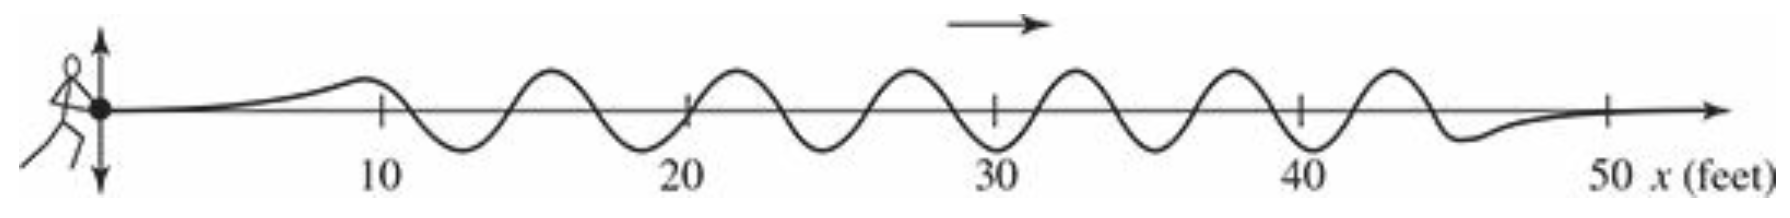
\includegraphics[width=0.6\linewidth]{uncertaintyPrinciplea.png}
            \caption{A wave with a (fairly) well-defined \emph{wavelength}, but an ill-defined \emph{position}.}
            \label{fig:uncertaintyPrinciplea}
        \end{subfigure}
        \begin{subfigure}[b]{\linewidth}
            \centering
            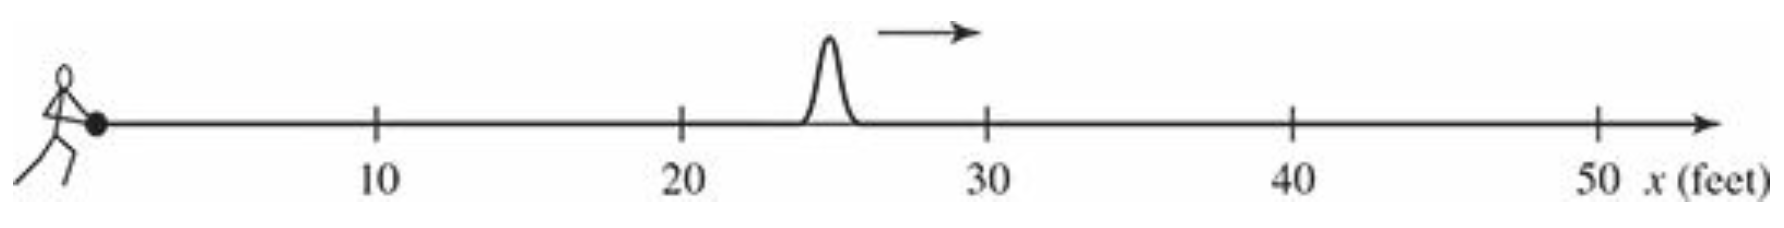
\includegraphics[width=0.6\linewidth]{uncertaintyPrincipleb.png}
            \caption{A wave with a (fairly) well-defined \emph{position}, but an ill-defined \emph{wavelength}.}
            \label{fig:uncertaintyPrincipleb}
        \end{subfigure}
        \caption{Visualizing the uncertainty principle.}
        \label{fig:uncertaintyPrinciple}
    \end{figure}
    \begin{itemize}
        \item Consider someone shaking a rope.
        \begin{itemize}
            \item If they do so a lot, you get a wave with a well-defined wavelength and ill-defined position.
            \item If they just shake it once, you get a wave with a well-defined position and ill-defined wavelength.
        \end{itemize}
        \item Thus, we see that there is a tradeoff between measuring the precision of wavelength and position.
        \item This discussion is adapted from a quantitative theorem of Fourier analysis that is beyond the scope of the book.
    \end{itemize}
    \item For a wave function, recall that de Brogelie said $\lambda\propto 1/p$, so the above relation between the uncertainties in position and wavelength becomes --- for a quantum particle --- a relation between the uncertainties in position and momentum.
    \item The Heisenberg Uncertainty Principle is stated, but not proven until Chapter 3.
\end{itemize}



\section{G Chapter 2: Time-Independent Schr\"{o}dinger Equation}
\emph{From \textcite{bib:Griffiths}.}
\subsection*{Section 2.1: Stationary States}
\begin{itemize}
    \item Goes through solving the TDSE via separation of variables.
    \begin{itemize}
        \item Remark: Separation of variables is "the physicist's first line of attack on any partial differential equation" \parencite[43]{bib:Griffiths}.
        \item \textcite{bib:Griffiths} finally addresses my criticism that separation of variables will restrict us to a tiny subset of solutions!
        \begin{itemize}
            \item Answer: This is true, but it just so happens that the solutions we \emph{do} get turn out to be of great interest. So essentially, this is "because it works" physics.
        \end{itemize}
    \end{itemize}
    \item \textbf{Time-independent Schr\"{o}dinger equation}: The equation defined as follows. \emph{Also known as} \textbf{TISE}. \emph{Given by}
    \begin{equation*}
        -\frac{\hbar^2}{2m}\dv[2]{\psi}{x}+V\psi = E\psi
    \end{equation*}
    \item The remaining sections of this chapter will focus on solving the TISE for various simple potentials.
    \item Three reasons why separable solutions are valuable.
    \begin{enumerate}
        \item They are \textbf{stationary states}.
        \begin{itemize}
            \item Every expectation value $\Exp{Q(x,p)}$ is also constant in time.
            \item In particular, $\Exp{\hat{\vec{x}}}$ is constant so $\Exp{\hat{\vec{p}}}=0$.
        \end{itemize}
        \item They are states of definite total energy.
        \begin{itemize}
            \item Reproves that $\sigma_H^2=0$, and hence every measurement of the total energy is certain to return the value $E$.
        \end{itemize}
        \item The general solution is a linear combination of separable solutions.
        \begin{itemize}
            \item Essentially, we can prove that \emph{every} solution to the TDSE can be written as
            \begin{equation*}
                \psi(x,t) = \sum_{n=0}^\infty c_n\psi_n(x)\e[-iE_nt/\hbar]
            \end{equation*}
        \end{itemize}
    \end{enumerate}
    \item \textbf{Stationary state}: A wave function $\psi(x,t)$ for which the probability density $|\psi(x,t)|^2$ does \emph{not} depend on $t$.
    \item Example: The linear combination of two stationary states produces motion.
    \begin{itemize}
        \item If $\psi(x,0)=c_1\psi_1(x)+c_2\psi_2(x)$, then we may compute that
        \begin{equation*}
            |\psi(x,t)|^2 = c_1^2\psi_1^2+c_2^2\psi_2^2+2c_1c_2\psi_1\psi_2\cos(\frac{E_2-E_1}{\hbar}t)
        \end{equation*}
    \end{itemize}
    \item $|c_n|^2$ is the probability that a measurement of the energy would return the value $E_n$.
    \begin{itemize}
        \item Proven in Chapter 3.
    \end{itemize}
    \item It follows from this understanding that we must have Wagner's favorite two equations,
    \begin{align*}
        \sum_{n=0}^\infty|c_n|^2 &= 1&
        \sum_{n=0}^\infty|c_n|^2E_n &= \Exp{\hat{H}}
    \end{align*}
    \item Remark: "Because the constants $\{c_n\}$ are independent of time, so too is the probability of getting a particular energy, and, \emph{a fortiori}, the expectation value of $H$. These are manifestations of energy conservation in quantum mechanics" \parencite[47]{bib:Griffiths}.
\end{itemize}




\end{document}